\section{Entwicklungsumgebung}
Da nun die zu verwendenden Technologien und Tools gewählt sind, kann mit der
eigentlichen Entwicklung des Prototypen begonnen werden. Als erster Schritt
muss die Entwicklungsumgebung gewählt und eingerichtet werden.

\subsection{Betriebssystem}
Privat und in meiner Firma arbeite ich mit dem Betriebssystem ``MacOS X'' von ``Apple'',
welches sich auch sehr gut für die Entwicklung von `Ruby on Rails' Webapplikationen
eignet, da ``Apple'' seit Version 10.4.6 von ``MacOS X'' `Ruby' und `Ruby on Rails' 
mitliefert \cite{macosx}.

Ich werden den Prototypen mit ``MacOS X'' Version 10.6.5 erstellen.

\subsection{Integrierte Entwicklungsumgebung}
Wenn man zum Beispiel eine Applikation mit `Java' entwickelt, wird sehr oft eine
sogenannte ``Integrierte Entwicklungsumgebung'' \cite{ide}, kurz `IDE', verwendet.
Diese bieten meist einen Texteditor, Compiler bzw. Interpreter, Linker, Debugger
und viele Quelltextformatierungsfunktionen.

Für die Entwicklung von `Ruby on Rails' Webapplikationen hat sich auf ``MacOS X''
jedoch schon sehr früh ein relativ einfacher und doch sehr hilfreicher Texteditor
namens ``Textmate'' durchgesetzt. Er wurde von Anfang an in den offiziellen Videotutorials 
von `rubyonrails.org' verwendet und auch Ryan Bates, eine Koryphäe in der
`Ruby on Rails' Welt, arbeitet ausschliesslich damit \cite{ryanbates}. 

Hinzu kommt das ``Terminal'', das Kommandozeilen-Programm von ``MacOS X'', mit
dem man den lokalen Webserver startet, diverse `Ruby on Rails' Skripte ausführt
und auch `Git', das Versionsverwaltungssystem, bedient.

Ich arbeite, um den Prototypen zu erstellen, mit ``Textmate'' Version 1.5.10
und dem ``Terminal'' Version 2.1.1.

\subsection{Versionsverwaltungssystem}
Ich habe mich entschlossen mit `Git' zu arbeiten und den Quellcode auf ``GitHub''
zur Verfügung zu stellen. Für den Prototypen möchte ich mit dem Standard
``Branching Model'' \cite{branching_model} arbeiten. Das bedeutet, dass ich
zwei der sogenannte Äste (``Branches'') führe. Einen für die Entwicklung namens 
`develop' und einen für die produktive Version namens `master'.

Wie dieses Modell funktioniert, wird in der Grafik \ref{branching_model} gut erklärt.
 
\begin{figure}[ht]
    \begin{center}
        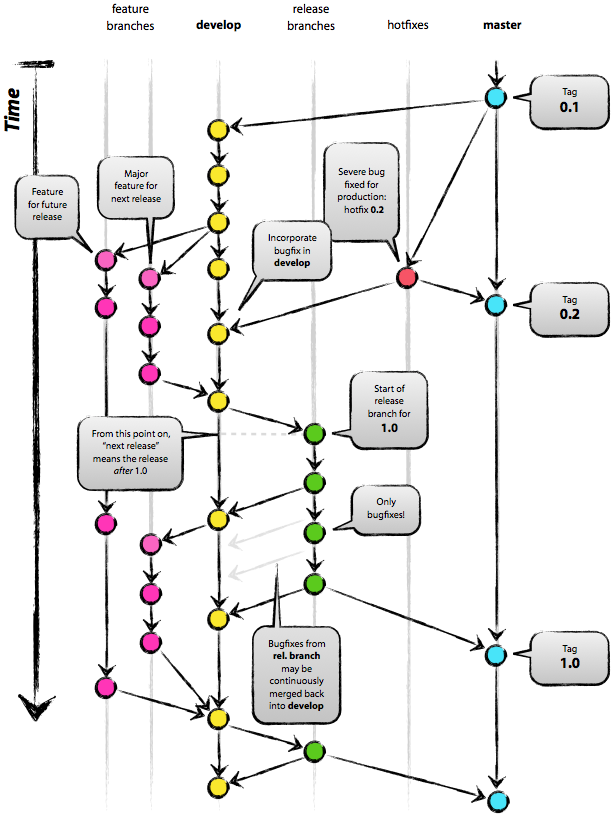
\includegraphics[width=1\textwidth,angle=0]{./bilder/branching_model.png}
        \caption{``A successful Git branching model'' von Vincent Driessen}
        \label{branching_model}
    \end{center}
\end{figure}

\clearpage

Ich habe hierzu einen privaten Account auf ``GitHub'' erstellt, welcher unter
\url{https://github.com/sspross} zu finden ist. Dieses Projekt ``OpenMediaLibrary''
habe ich unter \url{https://github.com/sspross/oml} eröffnet und öffentlich
verfügbar gemacht.

Wie das vorher erwähnte ``Branching Model'' dann in der Praxis aussieht, kann 
man auf der Grafik \ref{network_01} sehen.

\begin{figure}[ht]
    \begin{center}
        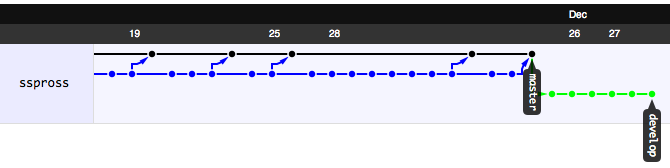
\includegraphics[width=0.8\textwidth,angle=0]{./bilder/network_01.png}
        \caption{Branches in der Praxis auf ``GitHub''}
        \label{network_01}
    \end{center}
\end{figure}

Die schwarze Linie ist der `master' Branch. Jeder schwarze Punkt widerspiegelt
einen produktiven Release, der in sich abgeschlossen ist und stabil läuft.

Die blaue Linie ist der `develop' Branch und jeder blaue Punkt stellt einen
Entwicklungsschritt dar, der jedoch nicht zwingend lauffähig, aber kompilierbar 
sein muss. Die grüne Linie ist ebenfalls der `develop' Branch und dient nur
der besseren Darstellung, bis er wieder in den `master' zurückgeführt wird.

Der vollständige und immer aktuelle Verlauf der Branches kann unter 
\url{https://github.com/sspross/oml/network} jederzeit eingesehen werden.

\section{Umsetzung}
Ich möchte in diesem Kapitel nicht auf die ganze Entstehung des Quellcodes 
eingehen, da dieser und dessen Verlauf vollständig auf ``GitHub'' unter
\url{https://github.com/sspross/oml} einsehbar ist.

Jedoch erläutere ich, welche Zusatzsoftware, auch genannt ``Plugins'' \cite{plugin}, ich 
verwendet habe und weshalb. Zusätzlich gehe ich auf grössere Herausforderungen,
die sich mir während der Entwicklung gestellt haben, ein und wie ich sie, wenn
überhaupt, gelöst habe.

\subsection{Zusatzsoftware}
In der nachstehenden Tabelle \ref{tab:plugins} liste ich die zusätzlich verwendeten
``Software'', geschrieben für das Framework `Ruby on Rails', auf und erläutere
ihren Verwendungszweck. Die Versionen sind als kurzer Hash \cite{hash} des
jeweiligen Projektes auf ``GitHub'' angegeben.

\begin{table}[ht]
\begin{center}
    \begin{tabular}{llp{6cm}lp{3cm}}
        \toprule Nr & Plugin & Verwendungszweck & Version & Herkunft \\
        \midrule 1 & project zero & Ein leeres `Ruby on Rails' 3.0 Template, welches
                 schon vorkonfigurierte Authentifizierungs-, Templating- und Testingfunktionen
                 mitliefert. & 8fb458c & \url{https://github.com/panter/project_zero} \\
        \midrule 2 & globalize3 & Bietet die Möglichkeit einfacher Objektinstanzen
                 zu internationalisieren. & aecb42f & \url{https://github.com/svenfuchs/globalize3} \\
        \midrule 3 & factory girl rails & Damit können Factories \cite{factory} für Tests
                 erstellt werden. & 5448687 & \url{https://github.com/thoughtbot/factory_girl_rails} \\
        \midrule 4 & resource controller & Hilft die Standard RESTful \cite{restful} Controller mit weniger Code
                 zu implementieren. & 48359da & \url{https://github.com/jamesgolick/resource_controller} \\
        \bottomrule
    \end{tabular}
    \caption{Verwendete ``Plugins'' und deren Verwendungszweck}
    \label{tab:plugins}
\end{center}
\end{table}

\clearpage

\subsection{Herausforderungen}
\subsubsection{Ruby on Rails Versionen}
Als ich begann den Prototypen zu Entwickeln verwendete ich die damals aktuelle
`Ruby on Rails' Version 2.3.4. Während der Weiterentwicklung gab es mehrere
Aktualisierungen von `Ruby on Rails' und ich musste auf die Version 2.3.8
updaten. Dies war kein Problem, da es sich dabei hauptsächlich um interne
Veränderungen von `Ruby on Rails' handelte, die nur einen minimalen Einfluss 
auf meinen bestehenden Quellcode hatten.

Gegen Mitte der Entwicklung erschien die `Ruby on Rails' Version 3.0 und wie
an der Versionsnummer schon zu erkennen ist, wurden darin Grundlegende Dinge
verändert und verbessert. Da ich den Anspruch erhebe, einen Prototypen zu schreiben
der auch von Drittentwicklern weiterentwickelt werden kann, musste ich meiner
Meinung nach zwingend auf die neue Version updaten, damit die Wahrscheinlichkeit
höher ist, zusätzliche Entwickler zu motivieren.

Dies stellte sich als nicht ganz einfach heraus. Als erstes Versuchte ich
den bestehenden Quellcode wie in den voran gegangenen Version einfach anzupassen.
Dies reichte jedoch nicht und endete in einer Sackgasse, die sich in meinem
Quellcode als eigener Branch widerspiegelt, der nicht wieder in den `develop'
Branch zurückgeführt wurde. Dies kann man aus der Grafik \ref{deadend} entnehmen.

\begin{figure}[ht]
    \begin{center}
        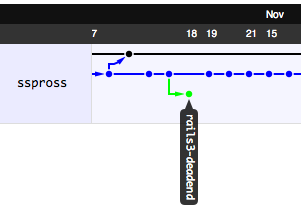
\includegraphics[width=0.3\textwidth,angle=0]{./bilder/deadend.png}
        \caption{Nicht zurückgeführter Branch `rails3-deadend'}
        \label{deadend}
    \end{center}
\end{figure}

Danach blieb mir nichts anderes übrig als den Quellcode nochmals neu auf einer
leeren `Ruby on Rails' 3.0 Instanz aufzubauen. Jedoch war es am Ende nur halb
so aufwändig, da sich in den Grundsätzen von `Ruby on Rails' nichts geändert 
hatte und somit der bestehende Code mehr oder weniger kopiert werden konnte.

Dazu hatte ich natürlich einen weiteren Branch namens `rails3' erstellt, der
dann wieder in den `develop' Branch zurückgeführt werden konnte, wie man
auf der Grafik \ref{rails3} erkennen kann.

\begin{figure}[ht]
    \begin{center}
        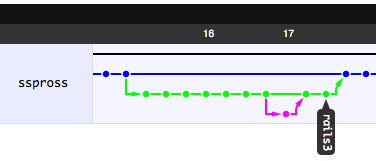
\includegraphics[width=0.4\textwidth,angle=0]{./bilder/rails3.png}
        \caption{Erfolgreich zurückgeführter Branch `rails3'}
        \label{rails3}
    \end{center}
\end{figure}

\clearpage

\subsubsection{Deplyoment}
Beim Deployment, auch ``Softwareverteilung'' \cite{deployment} genannt, stellte 
sich mir das Problem, dass ich lokal mit einer `SQlite' Datenbank entwickelt habe
und in der Produktion, also auf dem Zielserver wo dann der Prototyp installiert
wird, mit einer `mySQL' Datenbank arbeiten wollte.

`Ruby on Rails' unterstützt von Haus aus mehrere Verschiedene Datenbanktypen und
ist fähig mit `SQlite' und `mySQL' umzugehen. Jedoch ist `mySQL' abhängig vom
System, auf welchem es installiert wird.

Es war sehr viel Recherche nötig, aber am Schluss konnte ich, unteranderem mit
der Hilfe meines Betreuers, `mySQL' bei der Installation explizit deaktivieren,
damit auf dem Zielserver nicht versucht wird eine weiter `mySQL' Instanz zu
installieren. Zusätzlich konnte ich im sogenannten `Gemfile' elegant festlegen,
in welcher Umgebung welcher Datenbankadapter verwendet werden soll:

\begin{verbatim}
    group :development, :test do
      gem 'sqlite3-ruby'
    end
    
    group :production do
      gem 'mysql'
    end
\end{verbatim}

Dadurch wird definiert, dass bei einer lokalen Installation für die Entwicklungs-
(``Development'') und für die Testumgebung der `sqlite' Adapter und in der 
Produktionsumgebung (``Production'') der `mysql' Adapter verwendet wird.

\section{Testen}
Zu einem qualitativ hochwertigem Prototyp gehört, dass man ihn so gut wie 
möglich testet. Ich habe zwischen funktionalen Tests und sogenannten Unit-Tests
unterschieden und für beide mehrere Testfälle definiert.

Die funktionalen Tests simulieren Zugriffe eines Benutzers auf die Platttform.
Wie zum Beispiel ``Sich auf der Plattform anemlden'', ``Filme ansehen'', 
``Einen Film erstellen'' und ``Einen Film entfernen''.

Unit-Tests testen die Objekte bzw. Models der Applikation. Diese können in
`Ruby on Rails' in einer annähernd natürlich lesbaren Form geschrieben werden
und deshalb liste ich sie hier in der Dokumentation auf.

\subsection{Testfälle}
\subsubsection{Benutzer}
Ein vollständig abgefüllter Benutzer muss erfolgreich validiert werden können,
wenn man ihn speichert:

\begin{verbatim}
    context "Minimal User not saved" do
      setup { @user = Factory.build(:user) }
      should("validate") { assert @user.valid? }
    end
\end{verbatim}

Da die E-Mailadresse des Benutzers gleichzeitig seinen Benutzernamen darstellt,
muss sichergestellt werden, dass jede E-Mailadresse nur einmal verwendet werden
kann:

\begin{verbatim}
    context "Minimal user" do
      setup { @user = Factory(:user) }
      should validate_uniqueness_of(:email)
    end
\end{verbatim}

Wenn ein neuer Benutzer erstellt wird, dürfen noch keine Freundschaftsbeziehungen
bestehen und keine Bewertungen existieren:

\begin{verbatim}
    context "New user" do
      setup { @user = Factory(:user) }

      should "have no friends" do
        assert_equal @user.friends.size, 0
        assert_equal @user.inverse_friendships.size, 0
        assert_equal @user.direct_friends.size, 0
        assert_equal @user.inverse_friends.size, 0
        assert_equal @user.pending_friends.size, 0
        assert_equal @user.requested_friendships.size, 0
      end

      should "have no ratings" do
        assert_equal @user.ratings.size, 0
      end
    end
\end{verbatim}

\subsubsection{Bewertung}
Eine Bewertung muss einen gültigen Wert zwischen 1 und 10 enthalten:

\begin{verbatim}
    should "need a integer value between 1 and 10" do
      @rating.value = nil
      assert_equal @rating.valid?, false
      @rating.value = "adsf"
      assert_equal @rating.valid?, false
      @rating.value = 0
      assert_equal @rating.valid?, false
      @rating.value = 11
      assert_equal @rating.valid?, false
      @rating.value = 5
      assert_equal @rating.valid?, true
    end
\end{verbatim}

Ein Benutzer hat einen Film solange nicht bewertet, bis er ausdrücklich
eine Bewertung abgibt:

\begin{verbatim}
    should "be added to a movie and user" do
      assert_does_not_contain @silvan.ratings, @rating
      assert_does_not_contain @movie1.ratings, @rating
      assert_equal @movie1.ratings.size, 0
      assert_equal @silvan.ratings.size, 0
      assert_equal @rating.movie, nil
      assert_equal @rating.user, nil
      
      @rating.value = 5
      @rating.movie = @movie1
      @rating.user = @silvan
      @rating.save!
      
      @movie1.reload
      @silvan.reload
      
      assert_contains @silvan.ratings, @rating
      assert_contains @movie1.ratings, @rating
      assert_equal @movie1.ratings.size, 1
      assert_equal @silvan.ratings.size, 1
      assert_equal @rating.movie, @movie1
      assert_equal @rating.user, @silvan
    end
\end{verbatim}

Die Benutzer sehen verschiedene Bewertungen ihres Freundeskreises, da sie
verschiedene Freundschaften eingegangen sind:

\begin{verbatim}
    setup do 
      @silvan = Factory(:user)
      @stefan = Factory(:user)
      @friendship = Factory(:friendship, :user => @silvan, 
                            :friend => @stefan, :approved => true)
      @marcos = Factory(:user)
      @friendship = Factory(:friendship, :user => @marcos, 
                            :friend => @silvan, :approved => true)
      @muster = Factory(:user)
      @movie1 = Factory(:movie)
    end
    
    should "have different averages" do
      assert_equal @movie1.ratings.size, 0
      assert_equal @movie1.rating_all, nil
      assert_equal @movie1.rating_friends_of(@silvan), nil 
      assert_equal @movie1.rating_friends_of(@stefan), nil 
      assert_equal @movie1.rating_friends_of(@muster), nil 
      
      @movie1.ratings << Factory(:rating, :user => @silvan, :value => 4)
      assert_equal @movie1.ratings.size, 1
      assert_equal @movie1.rating_all, 4
      assert_equal @movie1.rating_friends_of(@silvan), nil 
      assert_equal @movie1.rating_friends_of(@stefan), 4 
      assert_equal @movie1.rating_friends_of(@muster), nil
      
      @movie1.ratings << Factory(:rating, :user => @muster, :value => 6)
      assert_equal @movie1.ratings.size, 2
      assert_equal @movie1.rating_all, 5
      assert_equal @movie1.rating_friends_of(@silvan), nil 
      assert_equal @movie1.rating_friends_of(@stefan), 4 
      assert_equal @movie1.rating_friends_of(@muster), nil
      
      @movie1.ratings << Factory(:rating, :user => @stefan, :value => 8)
      assert_equal @movie1.ratings.size, 3
      assert_equal @movie1.rating_all, 6
      assert_equal @movie1.rating_friends_of(@silvan), 8 
      assert_equal @movie1.rating_friends_of(@stefan), 4 
      assert_equal @movie1.rating_friends_of(@muster), nil
      
      @movie1.ratings << Factory(:rating, :user => @marcos, :value => 8)
      assert_equal @movie1.ratings.size, 4
      assert_equal @movie1.rating_all, 6.5
      assert_equal @movie1.rating_friends_of(@silvan), 8
      assert_equal @movie1.rating_friends_of(@stefan), 4 
      assert_equal @movie1.rating_friends_of(@muster), nil
      assert_equal @movie1.rating_friends_of(@marcos), 4
    end
\end{verbatim}

\subsubsection{Film}
Ein neuer Film hat zu beginn noch keine Bewertungen:

\begin{verbatim}
    should "have not any ratings first" do
      assert_does_not_contain @movie.ratings, @rating
      assert_equal @movie.ratings.size, 0
      assert_contains @user.ratings, @rating
    end
\end{verbatim}

Sobald ein Film bewertet wurde, kann kann ein Mittelwert der Bewertungen
berechnet werden:

\begin{verbatim}
    setup do
       @movie = Factory(:movie)
       @user = Factory(:user)
       @rating = Factory(:rating, :user => @user, :value => 5)
    end
    
    should "can get rated" do
      @movie.ratings << @rating
      @movie.save!
      
      assert_contains @movie.ratings, @rating
      assert_equal @movie.ratings.size, 1
      assert_equal @rating.movie, @movie
      assert_equal @movie.rating_all, 5
      assert_equal @movie.rating_friends_of(@user), nil
    end
\end{verbatim}

Wenn ein Film von der Plattform entfernt wird, werden auch die Bewertungen
der Benutzer entfernt:

\begin{verbatim}
    should "also destroy his ratings" do
      assert_contains Rating.all, @rating
      
      @movie.ratings << @rating
      @movie.save!
      assert_contains @movie.ratings, @rating
      
      @movie.destroy
      assert_does_not_contain Rating.all, @rating
    end
\end{verbatim}

\subsubsection{Freundschaft}
Zu Beginn sind zwei Personen nicht befreundet:

\begin{verbatim}
    should "have no friendship first" do
      assert_does_not_contain @stefan.friends, @silvan
      assert_does_not_contain @silvan.friends, @stefan
    end
\end{verbatim}

Eine Freundschaft kann von Seiten eines Benutzers beantragt werden:

\begin{verbatim}
    setup do
      @stefan = Factory(:user)
      @silvan = Factory(:user)
      @friendship = Factory(:friendship, :user => @silvan, :friend => @stefan)
    end
    
    should "can request a friendship" do
      assert_contains @silvan.pending_friends, @stefan
      assert_contains @stefan.requesting_friends, @silvan
    end
\end{verbatim}

Die Freundschaftsanfrage kann akzeptiert werden:

\begin{verbatim}
    should "can accept a friendship request" do
      request = @stefan.requested_friendships.first
      request.approved = true
      request.save!
      
      assert_contains @stefan.friends, @silvan
      assert_contains @silvan.friends, @stefan
      
      assert_does_not_contain @silvan.pending_friends, @stefan
      assert_does_not_contain @stefan.requesting_friends, @silvan
    end
\end{verbatim}

Die Freundschaft kann aber auch wieder aufgelöst werden:

\begin{verbatim}
    should "can end up with a friendship" do
      friendship = @stefan.inverse_friendships.first
      friendship.approved = false
      friendship.save!
      
      assert_does_not_contain @stefan.friends, @silvan
      assert_does_not_contain @silvan.friends, @stefan
      
      assert_contains @silvan.pending_friends, @stefan
      assert_contains @stefan.requesting_friends, @silvan 
    end
\end{verbatim}

\subsection{Testresultate}
Alle aufgeführten Unit-Testfälle und nicht aufgeführten funktionalen Testfälle
sind zum Zeitpunkt der Abgabe dieser Arbeit erfolgreich durchlaufen worden, 
wie man der Grafik \ref{testresultate} entnehmen kann.

\begin{figure}[ht]
    \begin{center}
        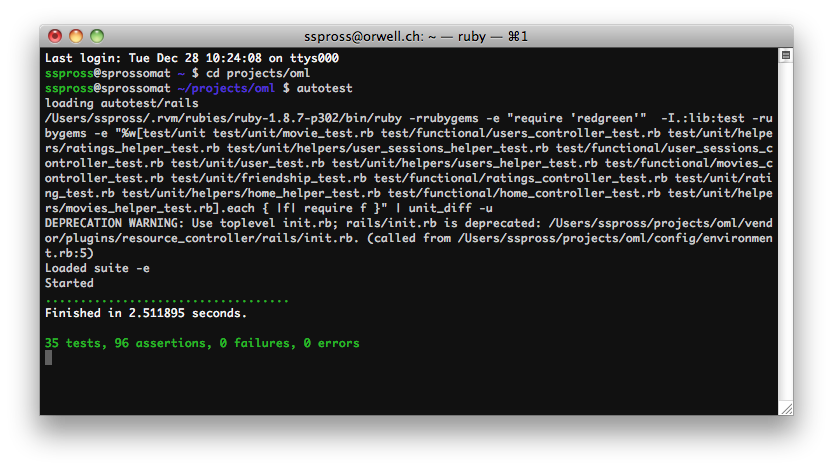
\includegraphics[width=0.9\textwidth,angle=0]{./bilder/testresultate.png}
        \caption{Testresultat vom 28.12.2010}
        \label{testresultate}
    \end{center}
\end{figure}